\documentclass[12pt]{article}

\usepackage{cmap}
\usepackage[T2A]{fontenc}
\usepackage[utf8]{inputenc}
\usepackage[russian]{babel}
\usepackage{graphicx}
\usepackage{amsthm,amsmath,amssymb}
\usepackage[russian,colorlinks=true,urlcolor=red,linkcolor=blue]{hyperref}
\usepackage{enumerate}
\usepackage{listings}
\usepackage{datetime}
\usepackage{wrapfig}
\usepackage{fancyhdr, graphicx}
\renewcommand{\headrulewidth}{0pt}
\fancyhead[L]{}
\fancyhead[R]{

\includegraphics[width=6cm]{img/logo.png}
}
\pagestyle{plain}
\title{\flushleft{Задача подструктурного поиска химического соединения}}
\date{}

\begin{document}

\maketitle
\thispagestyle{fancy}

\section{Введение}

Достижения в синтетической химии приводят к тому, что молекулы, синтезируемые в настоящее время, состоят из более сложных объектов с механическими связями и более обширных каркасов. Все более важным становится вопрос о том, как пользователи могут эффективно искать такие структуры в больших базах данных.

Задача поиска химических соединений, содержащих заданный фрагмент, в больших базах данных также является одной из задач в процессе разработки лекарств и позволяет решать конкретные проблемы при разработке новых лекарств. Рассмотрим на конкретном примере.

\begin{wrapfigure}{l}{0.5\textwidth}
    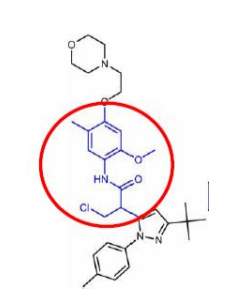
\includegraphics[width=0.35\textwidth]{img/abstract}
\end{wrapfigure}


Эта молекула является активной, но не может быть использована по причине:
\begin{itemize}
  \item фармакологических проблем (ADMET - absorption, distribution, metabolism, excretion and toxicity)
  \item защищенности патентом
\end{itemize}

Мы знаем что активность данной молекулы обусловлена выделенным фрагментом.

Значит существует вероятность найти активные молекулы среди ее производных, содержащих данный фрагмент.

\newpage
\section{Постановка задачи}

Рассмотрим химическое соединение $C$:

\begin{figure}[h]
  \label{figure:target}
  \center{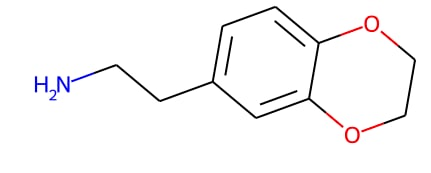
\includegraphics[height=3cm]{img/target}}
\end{figure}

Требуется разработать алгоритм, который будет находить все такие химические соединения $C^{'}$, в которых $C$ является подструктурой $C^{'}$:

\begin{figure}[h]
  \label{figure:result}
  \center{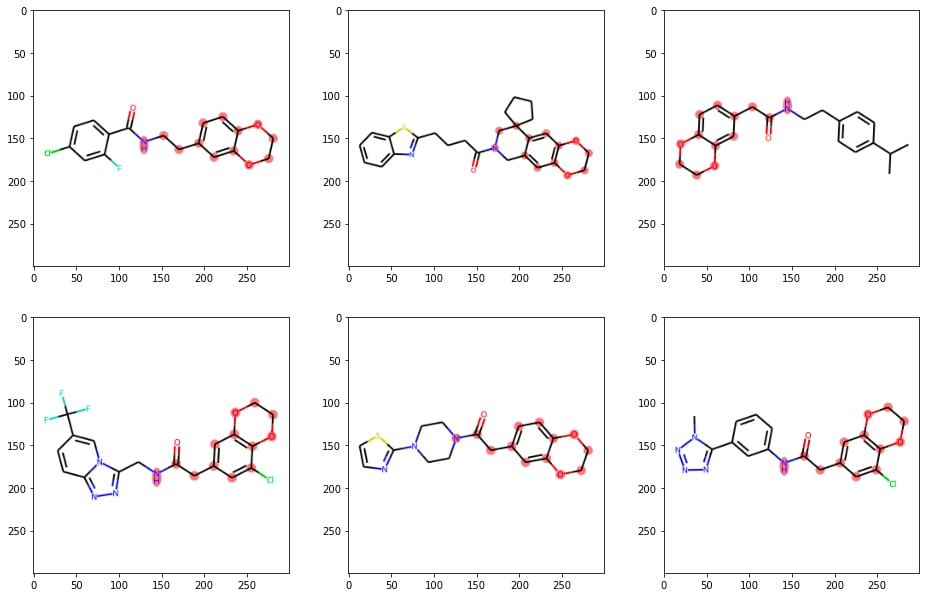
\includegraphics[width=1\linewidth]{img/result}}
\end{figure}

На данный момент база данных состоит из $10^9$ химических соединений. Ограничение на время поиска 1 секунда.
\end{document}
